\documentclass[aspectratio=169,10pt]{beamer}
\usetheme{Madrid}
\usecolortheme{seahorse}
\usefonttheme{professionalfonts}

\setbeamertemplate{footline}[frame number]
\setbeamertemplate{navigation symbols}{}

\usepackage{amsmath,amssymb,mathtools}
\usepackage{graphicx}
\usepackage{booktabs}
\usepackage{listings}
\usepackage{xcolor}
\usepackage{tikz}
\usetikzlibrary{arrows.meta,positioning}

\graphicspath{{figures/}}

\lstset{
  basicstyle=\ttfamily\scriptsize,
  numbers=left,
  numberstyle=\tiny,
  frame=single,
  backgroundcolor=\color{gray!7},
  commentstyle=\color{green!50!black}\itshape,
  keywordstyle=\color{blue!70!black}\bfseries,
  stringstyle=\color{orange!70!black},
  showstringspaces=false,
  breaklines=true,
  language=Python,
}

\newcommand{\R}{\mathbb{R}}
\newcommand{\E}{\mathbb{E}}
\newcommand{\Pb}{\mathbb{P}}
\newcommand{\Qb}{\mathbb{Q}}
\newcommand{\calK}{\mathcal{K}}
\newcommand{\calF}{\mathcal{F}}
\newcommand{\calP}{\mathcal{P}}
\newcommand{\calN}{\mathcal{N}}
\DeclareMathOperator*{\argmax}{arg\,max}

\title[E-Values -- Ch.8]{Hypothesis Testing with E-Values}
\subtitle{Chapter 8: Handling Multiple E-Values}
\author{Based on Ramdas \& Wang}
\date{}

\begin{document}

\begin{frame}
  \titlepage
\end{frame}

\begin{frame}[allowframebreaks]{Outline}
  \tableofcontents
\end{frame}

% ============================================================
\section{Setup and notation}
% ============================================================

\begin{frame}[allowframebreaks]{Why merge e-values at all?}
  \textbf{The setting.} We have $K \geq 2$ e-variables $E_1,\dots,E_K$, all valid for the \emph{same} null hypothesis. Write $\calK = \{1,\dots,K\}$.

  \vspace{0.3cm}
  \textbf{Where do multiple e-values come from?}
  \begin{itemize}
    \item Several analysts (or several methods) each produce their own e-value for the same question.
    \item Data splitting or sequential updating produces one e-value per chunk of data (Chapters 5, 7).
    \item Multiple testing: one e-value per hypothesis (Chapter 9) -- but this chapter is about combining e-values \emph{for one and the same hypothesis}.
  \end{itemize}

  \vspace{0.3cm}
  \textbf{The recurring question of this chapter:} given $E_1,\dots,E_K$, how do we combine them into a single e-value $F(E_1,\dots,E_K)$ that is itself valid -- i.e.\ still has expectation at most 1 under the null? The answer depends critically on what we are willing to assume about the \emph{dependence} between the $E_k$'s.

  \framebreak

  \textbf{Recall (from earlier chapters).} A random variable $E \geq 0$ is an \emph{e-variable} for a null hypothesis $\Pb$ if $\E^{\Pb}[E] \leq 1$ for every $\Pb$ in the null. Large values of $E$ are evidence against the null; we reject when $E \geq 1/\alpha$, which controls the type-I error at level $\alpha$ by Markov's inequality.

  \vspace{0.3cm}
  A key selling point of e-values (versus p-values) is that they are \emph{easy to combine} -- often without any assumption on how they depend on each other. This chapter makes that promise precise: it tells you exactly which combination rules are valid, depending on what you know about the dependence between $E_1,\dots,E_K$.
\end{frame}

\begin{frame}[allowframebreaks]{Notation you'll need}
  \begin{block}{Merging function}
    A function $F : [0,\infty)^K \to [0,\infty)$ that takes $K$ e-values as input and outputs a single combined value. We call $F$ \emph{valid} for a class of dependence structures if $F(E_1,\dots,E_K)$ is guaranteed to be an e-variable whenever $E_1,\dots,E_K$ are e-variables with that dependence structure.
  \end{block}

  \begin{block}{Arbitrary dependence}
    We make \emph{zero assumptions} about how $E_1,\dots,E_K$ relate to one another. They could be independent, could be identical copies of each other, could be adversarially correlated by some process we don't understand -- anything. A merging rule valid under arbitrary dependence must work no matter which of these is secretly true.
  \end{block}

  \begin{block}{FWER: family-wise error rate}
    When testing $K$ null hypotheses simultaneously and rejecting some subset, the FWER is $\Pb(\text{at least one rejected hypothesis is actually true})$. Controlling FWER at level $\alpha$ means this probability is $\leq \alpha$ no matter which hypotheses happen to be true.
  \end{block}

  \begin{block}{Martingale merging function (preview)}
    A merging function built by sequentially ``betting'' a fraction $\lambda_k$ of current capital on each new e-value, in the style of the testing-by-betting framework (Chapter 7). Valid whenever the e-values arrive \emph{sequentially} (each is unbiased given the past).
  \end{block}
\end{frame}

% ============================================================
\section{8.1 Merging e-values under arbitrary dependence}
% ============================================================

\begin{frame}[allowframebreaks]{8.1 Intuition: why averaging is the safe merge}
  \textbf{The puzzle.} If $E_1,\dots,E_K$ are each e-variables (each has mean $\leq 1$ under the null), which combinations of them are still guaranteed to have mean $\leq 1$ -- with \emph{no} assumption on their joint dependence?

  \vspace{0.2cm}
  \textbf{Sum?} No. $\E[E_1 + \cdots + E_K] = \E[E_1]+\cdots+\E[E_K] \leq K$, not $\leq 1$. If all $E_k$ happen to equal the same $E$, the sum is $KE$, which has mean up to $K$ -- badly invalid.

  \textbf{Max?} No. Even two e-values with mean $1$ each can be constructed so that $\max(E_1,E_2)$ has mean $>1$ (concentrating mass on the event where at least one is large).

  \textbf{Product?} Only under independence (Section 8.2) -- under arbitrary dependence it can blow up just like the sum.

  \textbf{Average?} \textbf{Yes -- always.} By linearity of expectation alone (which needs \emph{no} independence or dependence assumption whatsoever):
  \[
    \E\!\left[\frac{E_1+\cdots+E_K}{K}\right] = \frac{\E[E_1]+\cdots+\E[E_K]}{K} \leq \frac{1+\cdots+1}{K} = 1 .
  \]
  Linearity of expectation is the one identity in probability that \emph{never cares about dependence}: $\E[X+Y]=\E[X]+\E[Y]$ whether $X,Y$ are independent, identical, or adversarially entangled. Averaging exploits exactly this loophole -- it is the unique "linear" merge that is immune to dependence, which is why it (and its weighted variants) turn out to be the \emph{only} admissible choices in this fully-adversarial setting.
\end{frame}

\begin{frame}{Definition 8.1: e-merging functions}
  \begin{block}{E-merging function}
    An \emph{e-merging function} (of $K$ e-values) is an increasing Borel function
    \[
      F : [0,\infty)^K \to [0,\infty)
    \]
    such that, for \emph{any} null hypothesis and \emph{any} e-variables $E_1,\dots,E_K$ for it (with arbitrary, unknown joint dependence), $F(E_1,\dots,E_K)$ is again an e-variable.
  \end{block}
  \begin{itemize}
    \item \textbf{Symmetric}: $F(\mathbf{e})$ is unchanged by permuting the coordinates of $\mathbf{e}$ (treats all $K$ e-values interchangeably).
    \item \textbf{Dominates}: $F$ dominates $G$ if $F \geq G$ pointwise (strictly if also $F(\mathbf{e})>G(\mathbf{e})$ somewhere). $F$ is \emph{admissible} if no e-merging function strictly dominates it -- i.e.\ it can't be uniformly improved.
    \item \textbf{Essentially dominates}: $F$ essentially dominates $G$ if $G(\mathbf{e})>1 \implies F(\mathbf{e}) \geq G(\mathbf{e})$ -- $F$ is at least as good as $G$ whenever $G$'s output actually carries evidence ($>1$).
  \end{itemize}
\end{frame}

\begin{frame}{The arithmetic mean and its weighted versions}
  \begin{block}{Arithmetic mean $\mathbb{M}_K$}
    \[
      \mathbb{M}_K(e_1,\dots,e_K) = \frac{e_1+\cdots+e_K}{K}, \qquad e_1,\dots,e_K \in [0,\infty).
    \]
    Here $e_1,\dots,e_K$ are the realized e-values and $K$ is how many there are. This is an e-merging function under arbitrary dependence (shown above).
  \end{block}

  \begin{block}{Weighted arithmetic mean $\mathbb{M}_{\boldsymbol\lambda}$}
    For weights $\boldsymbol\lambda=(\lambda_1,\dots,\lambda_{K+1})$ in the simplex $\Delta_{K+1} = \{(x_1,\dots,x_{K+1}) \in [0,1]^{K+1} : \sum_k x_k = 1\}$,
    \[
      \mathbb{M}_{\boldsymbol\lambda}(e_1,\dots,e_K) = \sum_{k=1}^{K} \lambda_k e_k + \lambda_{K+1}.
    \]
    This mixes a weighted average of the e-values with a constant $1$ (weight $\lambda_{K+1}$ on "abstaining"); it is still an e-merging function under arbitrary dependence.
  \end{block}
  Geometric mean, harmonic mean, min: all valid too, but all are \emph{dominated by} $\mathbb{M}_K$ (see below) -- so there is never a reason to prefer them under arbitrary dependence.
\end{frame}

\begin{frame}[allowframebreaks]{Step-by-step: the average is an e-value, always}
  \textbf{Claim.} If $E_1,\dots,E_K$ are e-variables for a null $\Pb$ -- with \emph{any} joint dependence structure -- then $\mathbb{M}_K(E_1,\dots,E_K) = \tfrac{1}{K}\sum_k E_k$ is also an e-variable for $\Pb$.

  \vspace{0.2cm}
  \textbf{Step 1 (what we're given).} Each $E_k \geq 0$ and $\E^{\Pb}[E_k] \leq 1$. This is the \emph{only} thing we know -- we know nothing about $\mathrm{Cov}(E_i,E_j)$ or the joint law of $(E_1,\dots,E_K)$.

  \textbf{Step 2 (nonnegativity of the average).} Since each $E_k \geq 0$, the average $\tfrac{1}{K}\sum_k E_k \geq 0$ too. So it is a candidate e-variable (it's nonnegative, as required).

  \textbf{Step 3 (linearity of expectation -- the crucial step).} Expectation is linear \emph{regardless of dependence}:
  \[
    \E^{\Pb}\!\left[\frac{1}{K}\sum_{k=1}^K E_k\right] = \frac{1}{K}\sum_{k=1}^K \E^{\Pb}[E_k].
  \]
  This identity holds whether the $E_k$ are independent, identical, or adversarially dependent -- linearity of expectation never needs an independence assumption.

  \framebreak

  \textbf{Step 4 (plug in the bound).} Using $\E^{\Pb}[E_k]\leq 1$ for each $k$,
  \[
    \frac{1}{K}\sum_{k=1}^K \E^{\Pb}[E_k] \;\leq\; \frac{1}{K}\sum_{k=1}^K 1 \;=\; \frac{K}{K} \;=\; 1.
  \]

  \textbf{Step 5 (conclude).} Combining Steps 3--4, $\E^{\Pb}\!\left[\mathbb{M}_K(E_1,\dots,E_K)\right] \leq 1$, and by Step 2 it is nonnegative. Hence $\mathbb{M}_K(E_1,\dots,E_K)$ satisfies the definition of an e-variable for $\Pb$. Since $\Pb$ was an arbitrary null and $E_1,\dots,E_K$ were arbitrary e-variables (arbitrary dependence included), $\mathbb{M}_K$ is a valid e-merging function. $\blacksquare$

  \vspace{0.2cm}
  \textbf{Why this matters:} no other step used any structural assumption about the joint distribution -- the whole argument is "nonnegativity + linearity of expectation." That is exactly why averaging, uniquely among the natural combination rules, survives arbitrary dependence.
\end{frame}

\begin{frame}{Proposition 8.3: the mean is (essentially) the best symmetric rule}
  \begin{block}{Proposition 8.3}
    The arithmetic mean $\mathbb{M}_K$ essentially dominates any symmetric e-merging function: if a symmetric e-merging function $G$ ever outputs a value $>1$ (i.e.\ produces real evidence) at some input $\mathbf{e}$, then $\mathbb{M}_K(\mathbf{e}) \geq G(\mathbf{e})$.
  \end{block}

  \textbf{Proof sketch.} Suppose some symmetric $F$ beats $\mathbb{M}_K$ and also beats $1$ at some point $\mathbf{e}=(e_1,\dots,e_K)$: $b:=F(\mathbf e) > \max(\mathbb{M}_K(\mathbf e),1)=:a$. Let $\pi$ be a uniformly random permutation of $\calK$ and set $D_k = e_{\pi(k)}$ -- a random reshuffling of the same numbers. Each $D_k$ is itself an e-variable since $\E[D_k]=\mathbb{M}_K(\mathbf e)\leq a \leq 1$ after a suitable independent thinning by an event $A$ with $\Pb(A)=1/a$. By symmetry of $F$, $\E[F(D_1',\dots,D_K')] \geq b/a > 1$ -- contradicting that $F$ is a valid e-merging function. Hence no such $F$ exists.

  \vspace{0.2cm}
  \textbf{Theorem 8.4 (complete characterization).} $F$ is an \emph{admissible} e-merging function if and only if $F = \mathbb{M}_{\boldsymbol\lambda}$ for some $\boldsymbol\lambda \in \Delta_{K+1}$. In words: \emph{every} sensible way to merge arbitrarily dependent e-values is (dominated by) a weighted average with a constant.
\end{frame}

\begin{frame}[fragile]{Python: averaging survives adversarial dependence}
  \begin{lstlisting}
import numpy as np

rng = np.random.default_rng(0)
K, p, N = 5, 0.1, 20000

# Build K e-values that are STRONGLY DEPENDENT: they all move together
# via a shared latent shock W (fires with probability p).
a = np.array([8.0, 6.0, 10.0, 5.0, 9.0])     # values when shock hits
b = (1 - p * a) / (1 - p)                      # baseline (chosen so E[e_k]=1)

W = rng.binomial(1, p, size=N)
E = np.where(W[:, None] == 1, a, b)            # shape (N, K), all rows dependent

avg  = E.mean(axis=1)     # average across the K e-values, per trial
summ = E.sum(axis=1)
prod = E.prod(axis=1)

print("empirical mean of average:", avg.mean())   # ~1.00  (valid e-value!)
print("empirical mean of sum:    ", summ.mean())  # ~K     (invalid)
print("empirical mean of product:", prod.mean())  # >>1    (invalid, dependent)
  \end{lstlisting}
\end{frame}

\begin{frame}{Figure: averaging is safe, sum/product are not}
  \centering
  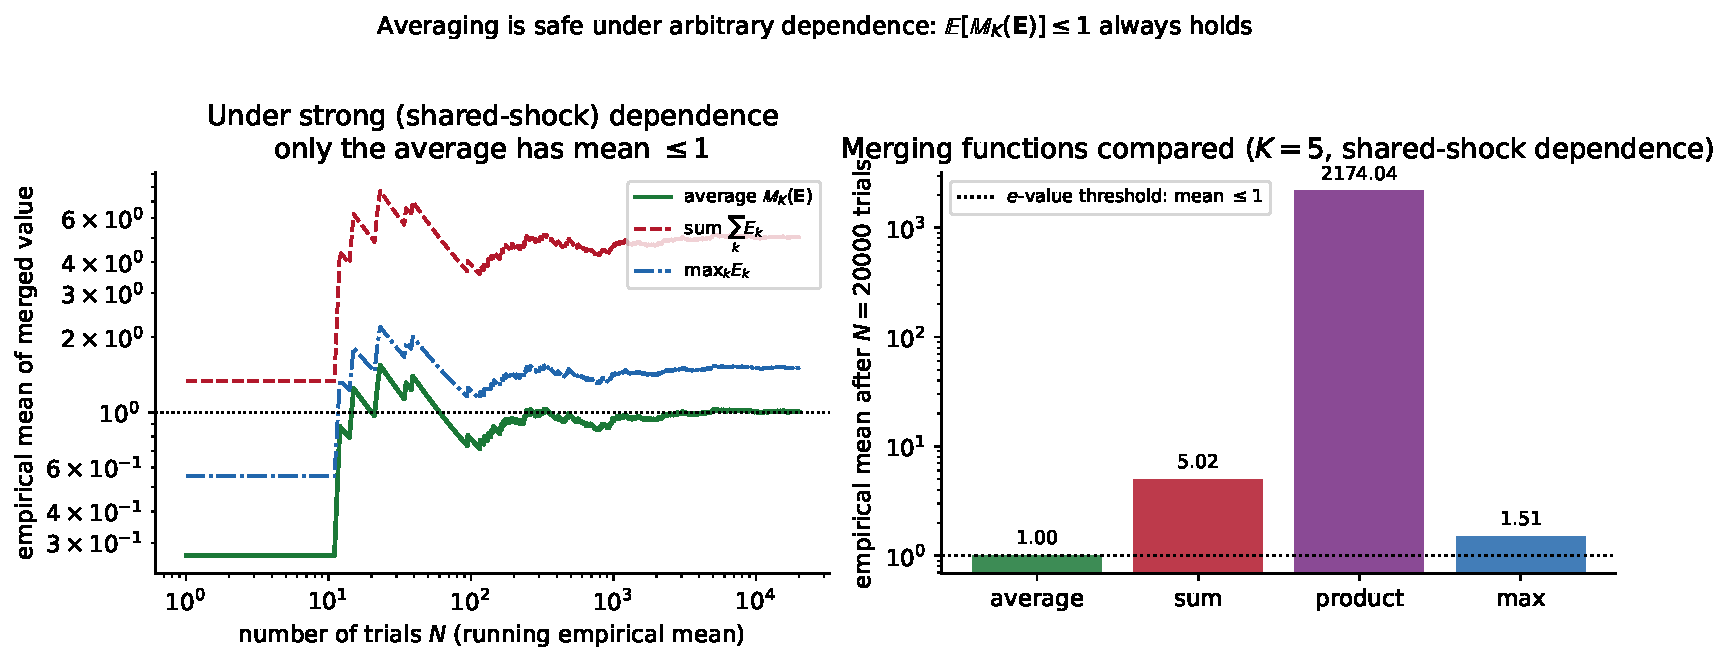
\includegraphics[width=0.98\textwidth]{fig_average_dependence.pdf}

  \small Under a shared-shock dependence structure ($K=5$, each $E_k$ individually has mean exactly 1), the empirical mean of the \emph{average} converges to $\leq 1$ (in fact $=1$), while the sum and product drift far above 1 -- they are not valid e-merging functions here.
\end{frame}

% ============================================================
\section{8.2 Independent e-values and their products}
% ============================================================

\begin{frame}{8.2 Intuition: independence buys you the product}
  Averaging was safe because it only used linearity of expectation. If we are additionally willing to assume $E_1,\dots,E_K$ are \emph{independent}, we unlock a stronger tool: the expectation of a \emph{product} of independent random variables factors:
  \[
    \E[E_1 \cdots E_K] = \E[E_1]\cdots\E[E_K] \leq 1 \cdots 1 = 1.
  \]
  This is the e-value analogue of Fisher's method for combining independent p-values. Under independence, the product is not just valid -- it is, in a precise sense, the "biggest" valid merge (Proposition 8.7 below). But bigger mean comes at a cost, which is exactly the subject of Section 8.4.
\end{frame}

\begin{frame}{Definition 8.5: ie-merging functions}
  \begin{block}{Ie-merging function}
    An \emph{ie-merging function} is a Borel function $F:[0,\infty)^K \to [0,\infty)$ such that $F(E_1,\dots,E_K)$ is an e-variable whenever $E_1,\dots,E_K$ are \emph{independent} e-variables (for any null). Unlike e-merging functions, $F$ need not be increasing in every coordinate.
  \end{block}

  \begin{block}{Product $\Pi_K$}
    \[
      \Pi_K(e_1,\dots,e_K) = \prod_{k=1}^K e_k, \qquad e_1,\dots,e_K \in [0,\infty).
    \]
  \end{block}

  \begin{block}{Proposition 8.6 (a simple admissibility check)}
    If $F$ is increasing and Borel and $\E^{\Pb}[F(\mathbf E)] = 1$ for \emph{every} vector of independent \emph{exact} e-variables $\mathbf E$ (exact meaning $\E[E_k]=1$, not just $\leq 1$), then $F$ is an admissible ie-merging function.
  \end{block}
  Since $\E[E_1\cdots E_K] = \prod_k \E[E_k] = 1$ for independent exact e-variables, $\Pi_K$ satisfies this and is admissible.
\end{frame}

\begin{frame}{U-statistics: interpolating between mean and product}
  \begin{block}{U-statistic merging functions}
    For $n \in \{0,1,\dots,K\}$,
    \[
      U_n(e_1,\dots,e_K) = \frac{1}{\binom{K}{n}}\sum_{A \subseteq \calK : |A|=n} \left(\prod_{k \in A} e_k\right).
    \]
    Here $U_n$ averages the size-$n$ subset-products over all $\binom{K}{n}$ subsets $A$ of size $n$.
  \end{block}
  \begin{itemize}
    \item $n=K$: only one subset ($A=\calK$), so $U_K = \Pi_K$, the full product.
    \item $n=1$: averages single e-values, so $U_1 = \mathbb{M}_K$, the arithmetic mean.
    \item $n=0$: the empty product is 1, so $U_0 \equiv 1$ (the trivial, always-valid e-value).
    \item Convex mixtures $\sum_n c_n U_n$ ($c_n \geq 0$, $\sum_n c_n=1$) are also admissible ie-merging functions (by Prop.\ 8.6).
  \end{itemize}
  \textbf{Not a complete class:} Example 8.8 in the book exhibits an admissible ie-merging function, $f(e_1,e_2) = \tfrac12\left(\tfrac{e_1}{1+e_1}+\tfrac{e_2}{1+e_2}\right)(1+e_1e_2)$, that is \emph{not} any convex mixture of the $U_n$'s -- so, unlike the arbitrary-dependence case, there is no simple complete characterization here.
\end{frame}

\begin{frame}{Proposition 8.7: the product is (weakly) optimal}
  \begin{block}{Proposition 8.7}
    The product $\Pi_K$ weakly dominates any ie-merging function $F$: for all $(e_1,\dots,e_K) \in [1,\infty)^K$ (i.e.\ whenever \emph{every} input already carries some evidence, $e_k \geq 1$),
    \[
      F(e_1,\dots,e_K) \leq \Pi_K(e_1,\dots,e_K) = e_1 \cdots e_K.
    \]
  \end{block}
  \textbf{Why only on $[1,\infty)^K$?} With a large $K$, it is rare that \emph{all} inputs exceed 1 simultaneously, so this is a genuinely weak requirement -- much weaker than full domination on all of $[0,\infty)^K$.

  \vspace{0.2cm}
  \textbf{Beyond independence: negative dependence also works.} If $E_1,\dots,E_K$ are \emph{negative lower orthant dependent} (NLOD), meaning
  \[
    \Pb\Big(\bigcap_{k \in \calK} \{E_k \leq x_k\}\Big) \leq \prod_{k \in \calK} \Pb(E_k \leq x_k) \quad \text{for all } (x_1,\dots,x_K),
  \]
  then $\Pi_K$ (and the $U_n$'s) remain valid e-merging functions even though $E_1,\dots,E_K$ are not independent -- NLOD is a weaker, one-directional relaxation of independence (equality in (8.5) recovers exact independence).
\end{frame}

\begin{frame}[fragile]{Python: 8.2 -- product needs independence}
  \begin{lstlisting}
import numpy as np
rng = np.random.default_rng(1)

K, N = 5, 20000

# INDEPENDENT e-values: each E_k = 2*Bernoulli(1/2), mean = 1 exactly.
E_indep = 2 * rng.binomial(1, 0.5, size=(N, K))
prod_indep = E_indep.prod(axis=1)
print("independent product, empirical mean:", prod_indep.mean())   # ~1.0 (valid)

# DEPENDENT e-values built as identical COPIES: E_k = E for all k.
E_shared = 2 * rng.binomial(1, 0.5, size=(N, 1))
E_copies = np.repeat(E_shared, K, axis=1)
prod_copies = E_copies.prod(axis=1)
print("copied (dependent) product, empirical mean:", prod_copies.mean())
# ~ 2^{K-1}, badly invalid -- independence was doing all the work above
  \end{lstlisting}
\end{frame}

% ============================================================
\section{8.3 Sequential e-values and martingale merging functions}
% ============================================================

\begin{frame}{8.3 Intuition: e-values that arrive one at a time}
  Independence is a strong, static assumption about $K$ e-values considered jointly. A more flexible and dynamic notion: e-values that arrive \emph{sequentially}, where each new one is only required to be "fair" (mean $\leq 1$) \emph{given everything seen so far} -- exactly like a fair bet on the next round of a game, regardless of how earlier rounds went. This generalizes independence (independent e-values are automatically sequential) and connects directly to the testing-by-betting framework of Chapter 7.
\end{frame}

\begin{frame}{Definition 8.9: sequential e-values, se-merging functions}
  \begin{block}{Sequential e-values}
    $E_1,\dots,E_K$ are \emph{sequential} for a class of nulls $\calP$ if, for every $\Pb \in \calP$ and every $k \in \calK$,
    \[
      \E^{\Pb}[E_k \mid E_1,\dots,E_{k-1}] \leq 1.
    \]
    That is: conditional on everything observed before round $k$, the next e-value $E_k$ is still (conditionally) a valid e-variable. This is strictly more general than independence.
  \end{block}
  \begin{block}{Se-merging function}
    A Borel $F:[0,\infty)^K \to [0,\infty)$ such that $F(E_1,\dots,E_K)$ is an e-variable for \emph{any} sequential e-variables $E_1,\dots,E_K$. \emph{Exact} if $F(\mathbf E)$ is exact (mean $=1$) whenever the inputs are exact and sequential.
  \end{block}
  All convex mixtures of the U-statistics $U_n$ (including $\mathbb{M}_K$ and $\Pi_K$) are se-merging functions, since independent e-values are automatically sequential.
\end{frame}

\begin{frame}{Definition 8.10: martingale merging functions}
  \begin{block}{Martingale merging function}
    $F$ is a \emph{martingale merging function} if
    \[
      F(e_1,\dots,e_K) = \prod_{k=1}^K \left(1 - \lambda_k + \lambda_k e_k\right),
    \]
    where $\lambda_1 \in [0,1]$ is a fixed constant and, for $k \geq 2$, $\lambda_k = \lambda_k(e_1,\dots,e_{k-1}) \in [0,1]$ is allowed to depend on the e-values seen \emph{before} round $k$.
  \end{block}
  \textbf{Betting interpretation.} Think of capital that starts at 1. At round $k$, you bet a \emph{fraction} $\lambda_k$ of your current capital on the outcome $E_k$: if the bet were fully committed you'd multiply by $e_k$, but betting only a fraction $\lambda_k$ of capital gives the factor $(1-\lambda_k) + \lambda_k e_k$ (keep $1-\lambda_k$ untouched, multiply $\lambda_k$ by $e_k$). Multiplying these factors across rounds tracks total capital.
  \begin{itemize}
    \item $\lambda_k \equiv 1/K$ for all $k$ recovers (a variant connected to) the arithmetic mean -- betting a \emph{fixed amount}, not a fixed proportion, each round.
    \item $\lambda_k \equiv 1$ for all $k$ recovers the product $\Pi_K$ -- "all-in" every round.
  \end{itemize}
\end{frame}

\begin{frame}{Proposition 8.11 and Theorem 8.12}
  \begin{block}{Proposition 8.11}
    Any martingale merging function is an exact se-merging function. Moreover, a convex combination of martingale merging functions is again a martingale merging function.
  \end{block}
  \textbf{Proof idea (backward induction).} Write $L_k = \lambda_k(E_1,\dots,E_{k-1})$. Conditioning on the past up to round $K-1$:
  \[
    \E^{\Pb}[F(E_1,\dots,E_K) \mid \calF_{K-1}] = F(E_1,\dots,E_{K-1},1)\big(1 - L_K + L_K \,\E^{\Pb}[E_K\mid \calF_{K-1}]\big) \leq F(E_1,\dots,E_{K-1},1),
  \]
  using $\E^{\Pb}[E_K \mid \calF_{K-1}] \leq 1$ and $L_K \in [0,1]$. Peel off rounds $K, K-1, \dots, 1$ this way to get $\E^{\Pb}[F(E_1,\dots,E_K)] \leq F(1,\dots,1) = 1$.

  \begin{block}{Theorem 8.12 (completeness)}
    Every se-merging function is dominated by \emph{some} martingale merging function. So, just as $\mathbb{M}_{\boldsymbol\lambda}$ completely characterizes admissible merges under arbitrary dependence, martingale merging functions completely characterize (up to domination) valid merges of sequential e-values.
  \end{block}
\end{frame}

\begin{frame}{Examples: hit-and-stop, and the empirically adaptive process}
  \begin{block}{Example 8.13: hit-and-stop}
    Fix a level $\alpha \in (0,1)$. As soon as the running combined value $F(e_1,\dots,e_k,1,\dots,1)$ first reaches $1/\alpha$ (i.e.\ we could already reject), set all future $\lambda_j=0$ -- stop betting. This makes $F$ \emph{non-monotonic} in general (an early win can be "locked in" rather than risked later), which is perfectly fine: martingale merging functions need not be increasing, only \emph{sequentially} monotone (increasing in $e_k$ holding future e-values at their neutral value $1$).
  \end{block}
  \begin{block}{Example 8.14: empirically adaptive e-process}
    Choose $\lambda_k$ at each round by optimizing the log-growth of capital \emph{so far}:
    \[
      \lambda_k(e_1,\dots,e_{k-1}) = \argmax_{\lambda \in [0,\gamma]} \frac{1}{k-1}\sum_{s=1}^{k-1} \log\big((1-\lambda)+\lambda e_s\big), \qquad \gamma \in (0,1].
    \]
    A data-driven, default choice with no prior knowledge of the alternative required -- and it is asymptotically log-optimal (Theorem 7.22).
  \end{block}
\end{frame}

\begin{frame}[fragile]{Python: 8.3 -- a martingale merging function in action}
  \begin{lstlisting}
import numpy as np

def martingale_merge(e, lam):
    """F(e_1,...,e_K) = prod_k (1 - lam_k + lam_k * e_k)."""
    e = np.asarray(e, dtype=float)
    lam = np.asarray(lam, dtype=float)
    return np.prod(1 - lam + lam * e)

e = [0.8, 1.3, 2.1, 0.5, 1.8]           # our running example (see next slide)

# Fixed-fraction betting, lambda_k = 1/K for all k (mean-like betting):
lam_fixed = [1/5]*5
print("fixed 1/K betting:", martingale_merge(e, lam_fixed))

# All-in every round (lambda_k = 1), i.e. this equals the raw product:
lam_allin = [1.0]*5
print("all-in (= product):", martingale_merge(e, lam_allin), "vs prod:", np.prod(e))
  \end{lstlisting}
\end{frame}

% ============================================================
\section{Running numerical example}
% ============================================================

\begin{frame}{Running example: 5 correlated tests of the SAME coin}
  \textbf{Setup.} We suspect one coin is unfair, and we run $K=5$ different tests of the very same coin (e.g. 5 different statisticians, or 5 different test statistics, applied to the same sequence of flips). Because they all use the \emph{same underlying coin and data}, the resulting e-values are genuinely, unavoidably \textbf{dependent} -- there is no reason to assume independence here.
  \[
    e_1 = 0.8, \quad e_2 = 1.3, \quad e_3 = 2.1, \quad e_4 = 0.5, \quad e_5 = 1.8.
  \]
  \textbf{Average (by hand):}
  \[
    \mathbb{M}_5(\mathbf e) = \frac{0.8+1.3+2.1+0.5+1.8}{5} = \frac{6.5}{5} = 1.3.
  \]
  \textbf{Product (by hand):}
  \[
    \Pi_5(\mathbf e) = 0.8 \times 1.3 \times 2.1 \times 0.5 \times 1.8 = 1.9656.
  \]
  Numerically the product ($1.9656$) is larger than the average ($1.3$) -- more "evidence," at first glance.
\end{frame}

\begin{frame}{Running example: which merge is actually valid here?}
  \begin{itemize}
    \item \textbf{The average, $1.3$, is a valid e-value regardless of the dependence between the 5 tests.} By Section 8.1's argument (linearity of expectation only), $\mathbb{M}_5(\mathbf E)$ has mean $\leq 1$ under the null no matter how the 5 tests on the same coin are correlated. We may safely report $1.3$ as combined evidence and, e.g., reject at level $\alpha$ if $1.3 \geq 1/\alpha$ (here, $\alpha \leq 1/1.3 \approx 0.77$ -- weak evidence, appropriately modest given the redundancy across 5 dependent tests of one coin).
    \item \textbf{The product, $1.9656$, is \emph{not} justified here.} Section 8.2's guarantee for the product requires independent (or at least NLOD) e-values. Since all 5 tests examine the very same coin and data, treating them as independent would double-count the same evidence 5 times over -- the product could then wildly overstate the evidence (recall Section 8.1's dependence simulation, where an analogous product's empirical mean blew up past $2000$).
  \end{itemize}
  \begin{block}{Takeaway}
    Numerically, product $>$ average here ($1.9656 > 1.3$), but only the average carries a valid statistical guarantee under the (realistic) dependence of this example. Reporting the product would be an invalid, overconfident use of e-value theory.
  \end{block}
\end{frame}

\begin{frame}[fragile]{Python: the running example, verified}
  \begin{lstlisting}
import numpy as np

e = np.array([0.8, 1.3, 2.1, 0.5, 1.8])
K = len(e)

avg  = e.mean()          # valid regardless of dependence (Section 8.1)
prod = e.prod()          # valid ONLY if the 5 tests are independent (Section 8.2)

print(f"average = {avg}")   # 1.3
print(f"product = {prod}")  # 1.9656

alpha_avg = 1/avg
print(f"average rejects for alpha >= {alpha_avg:.3f}")   # alpha >= 0.769

# The product looks stronger, but on the SAME coin's data the 5 tests are
# dependent, so we have NO guarantee that E[prod] <= 1 -- only the
# average carries a distribution-free guarantee here.
  \end{lstlisting}
\end{frame}

% ============================================================
\section{8.4 Mean-variance trade-off}
% ============================================================

\begin{frame}{8.4 Intuition: bigger mean is not free}
  Proposition 8.7 says the product $\Pi_K$ weakly dominates every ie-merging function -- so isn't the product simply "the best" choice under independence? \textbf{No.} Under the alternative hypothesis $\Qb$ (where we \emph{want} large e-values), the product does have the largest possible expectation among se-merging functions applied to "powered" e-values ($\E^{\Qb}[E_k]\geq 1$) -- but a large mean can be driven almost entirely by a vanishingly rare, enormous outcome, while the \emph{typical} realization is disappointing (even $0$). This is the classic mean-variance trade-off: the product maximizes the mean but also (weakly) maximizes the variance among exact se-merging functions.
\end{frame}

\begin{frame}{Proposition 8.16: moments are maximized by the product}
  \begin{block}{Lemma 8.15}
    If $F$ is an ie-merging function and $a \geq 1$, then $G(e_1,\dots,e_K) = F(ae_1,e_2,\dots,e_K)/a$ is also an ie-merging function. (Rescaling one coordinate by $a\geq1$ and dividing the output by $a$ preserves validity.)
  \end{block}
  \begin{block}{Proposition 8.16}
    Let $F$ be an se-merging function. For independent, nonnegative $E_1,\dots,E_K$ under an alternative $\Qb$ with $\E^{\Qb}[E_k]\geq 1$ for each $k$, and for every moment order $m \in [1,\infty)$:
    \[
      \E^{\Qb}\big[F(E_1,\dots,E_K)^m\big] \;\leq\; \prod_{k=1}^K \E^{\Qb}[E_k^m] \;=\; \E^{\Qb}\big[\Pi_K(E_1,\dots,E_K)^m\big].
    \]
    In particular (taking $m=2$, exact e-variables), $\mathrm{var}^{\Pb}(F(\mathbf E)) \leq \mathrm{var}^{\Pb}(\Pi_K(\mathbf E))$: \textbf{the product has the largest variance among all exact se-merging functions.}
  \end{block}
  So: the product maximizes \emph{every} moment (mean, variance, everything) among se-merging functions applied to independent, powered e-values -- but a large variance is generally undesirable, since it means the outcome is unreliable.
\end{frame}

\begin{frame}{Example 8.17: all-in versus log-optimal}
  Suppose (under $\Qb$) each $E_k$, $k=1,2,\dots$, independently takes value $4$ w.p.\ $1/2$ and $0$ w.p.\ $1/2$ (so $\E^{\Qb}[E_k]=2$, a genuinely powered e-value).
  \begin{itemize}
    \item \textbf{All-in strategy} ($\lambda_k \equiv 1$, i.e.\ the raw product): $M_k^{\text{all-in}} = \Pi_k(E_1,\dots,E_k) = 4^k$ w.p. $2^{-k}$, and $=0$ w.p.\ $1-2^{-k}$. Its mean $\E^{\Qb}[M_k^{\text{all-in}}] = 2^k$ is the \emph{largest possible} -- but $M_k^{\text{all-in}} \to 0$ almost surely as $k\to\infty$: the strategy is a near-certain wipeout that happens to have an astronomically lucky tail.
    \item \textbf{Log-optimal strategy} ($\lambda_k \equiv 1/3$, the growth-rate maximizer): $M_k^\ast$ grows like $(4/3)^k$ almost surely (law of large numbers) -- slower in expectation, but reliable: it doesn't collapse to 0.
  \end{itemize}
  \begin{block}{Moral}
    E-power (Chapter 7) is measured by the expected \emph{logarithm} under $\Qb$, not by any raw moment. The all-in/product strategy wins on every moment yet loses on the metric that actually matters for a useful, repeatable procedure.
  \end{block}
\end{frame}

\begin{frame}[fragile]{Python: 8.4 -- product vs.\ average, mean-variance trade-off}
  \begin{lstlisting}
import numpy as np
rng = np.random.default_rng(2)

N, Kmax = 4000, 25
draws = rng.binomial(1, 0.5, size=(N, Kmax))     # 1 = "high" outcome (e_k = 4)
e_vals = np.where(draws == 1, 4.0, 0.0)          # each e_k has mean 2

for K in [1, 5, 10, 25]:
    e_K = e_vals[:, :K]
    prod_K, avg_K = e_K.prod(axis=1), e_K.mean(axis=1)
    theory_mean_prod = 2.0**K                       # exact, not simulated
    print(f"K={K:2d}  E[prod] (exact)={theory_mean_prod:.3g}  "
          f"median(prod)={np.median(prod_K):.3g}  "
          f"mean(avg)={avg_K.mean():.3g}  P(prod=0)={np.mean(prod_K==0)*100:.1f}%")
# The product's mean explodes exponentially, yet its typical (median)
# value is 0 with probability -> 1: the average is the "reliable" merge.
  \end{lstlisting}
\end{frame}

\begin{frame}{Figure: the mean-variance trade-off}
  \centering
  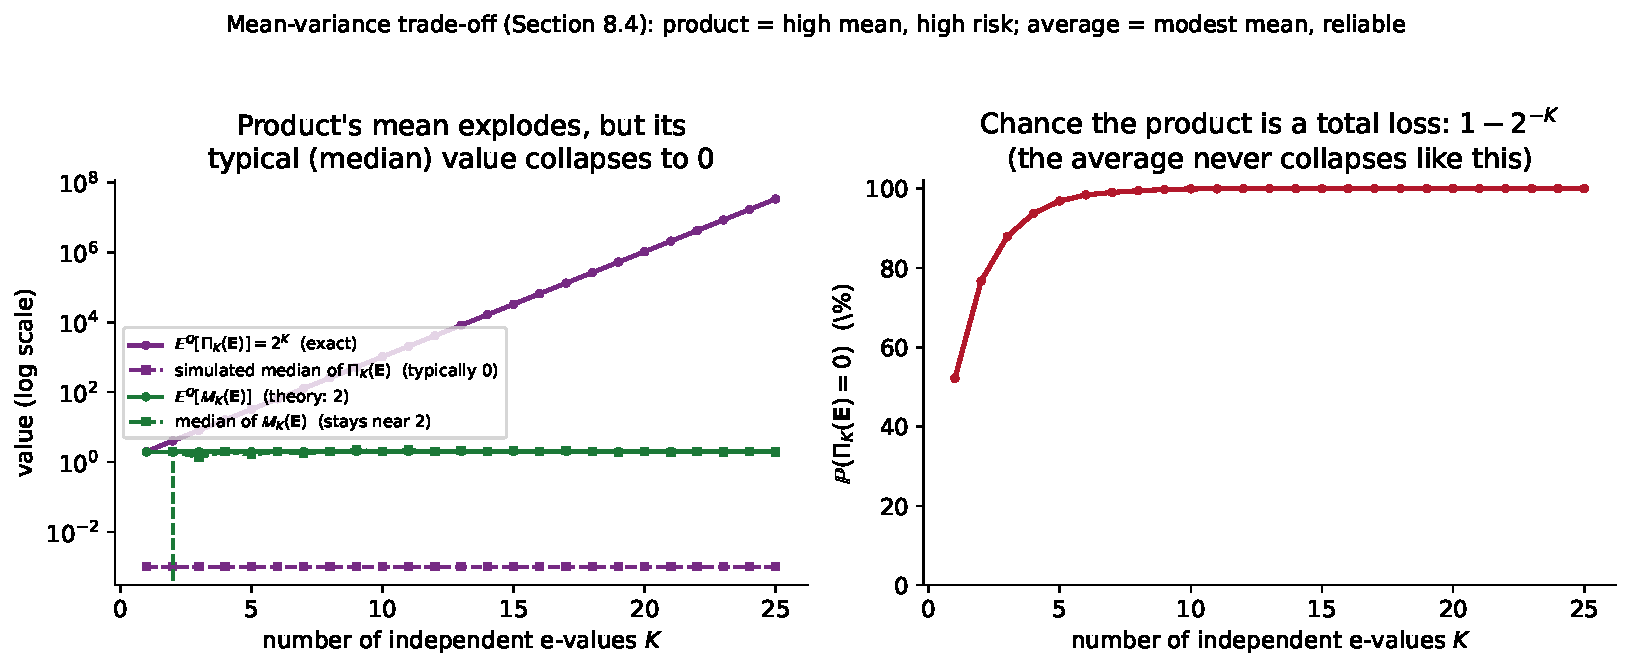
\includegraphics[width=0.98\textwidth]{fig_product_vs_average.pdf}

  \small Left: the product's exact mean $2^K$ (theory) explodes exponentially, while its simulated \emph{median} collapses to (essentially) $0$; the average's mean and median both stay near $2$. Right: the probability that the product is a total loss ($=0$) tends to $1$ as $K$ grows -- a risk the average never carries.
\end{frame}

% ============================================================
\section{8.5 Family-wise error rate and merging e-values}
% ============================================================

\begin{frame}{8.5 Intuition: from merging to multiple testing}
  Now suppose $E_1,\dots,E_K$ are e-values for $K$ \emph{different} null hypotheses $\calP_1,\dots,\calP_K$ (rather than $K$ e-values for one hypothesis). We want a testing procedure that outputs a set of rejected hypotheses $\mathcal D \subseteq \calK$ while controlling the \textbf{family-wise error rate (FWER)}: the chance of even a single false rejection, however many hypotheses are actually true.
  \[
    \Pb(\mathcal D \cap \calN \neq \varnothing) \leq \alpha \quad \text{for every possible } \Pb,
  \]
  where $\calN = \{k \in \calK : \Pb \in \calP_k\}$ is the (unknown) set of hypotheses that happen to be true. The merging tools from 8.1--8.4 turn out to give a simple, general recipe for this.
\end{frame}

\begin{frame}{The mean e-collection and its FWER guarantee}
  For any subset $A \subseteq \calK$, merge the e-values of hypotheses in $A$ into a single e-value for the \emph{intersection null} $\bigcap_{k \in A} \calP_k$. Using the arithmetic mean (valid under arbitrary dependence -- we don't know how $E_1,\dots,E_K$ relate across hypotheses):
  \begin{block}{Mean e-collection (8.11)}
    \[
      E_A = \frac{1}{|A|}\sum_{k \in A} E_k, \qquad A \subseteq \calK.
    \]
    $E_A$ is a valid e-variable for $\bigcap_{k\in A}\calP_k$ for every subset $A$ simultaneously (by the Section 8.1 argument, applied separately to each $A$).
  \end{block}
  \begin{block}{The e-testing procedure}
    Define $E_k^\ast = \min_{A \subseteq \calK : k \in A} E_A$ (the smallest merged value over all subsets containing $k$), and reject $k$ whenever $E_k^\ast \geq 1/\alpha$.
  \end{block}
\end{frame}

\begin{frame}{Why this controls FWER: a two-line argument}
  \textbf{Claim:} the rule "reject $k$ iff $E_k^\ast \geq 1/\alpha$" controls FWER at level $\alpha$.

  \vspace{0.2cm}
  \textbf{Step 1.} For any true null index $k \in \calN$ and \emph{any} $A \ni k$ with $A$ possibly restricted to $\calN$: since $A \subseteq \calN$ is available as a candidate (in particular $A = \calN$), $E_k^\ast = \min_{A \ni k} E_A \leq E_\calN$. Taking the max over $k \in \calN$:
  \[
    \max_{k \in \calN} E_k^\ast \;\leq\; E_\calN.
  \]

  \textbf{Step 2 (Markov's inequality).} $E_\calN$ is a genuine e-variable for $\bigcap_{k\in\calN}\calP_k$ (the truth), so $\Pb(E_\calN \geq 1/\alpha) \leq \alpha \cdot \E[E_\calN] \leq \alpha$.

  \textbf{Conclusion.}
  \[
    \Pb(\mathcal D \cap \calN \neq \varnothing) = \Pb\Big(\max_{k \in \calN} E_k^\ast \geq 1/\alpha\Big) \leq \Pb(E_\calN \geq 1/\alpha) \leq \alpha.
  \]
  This works for \emph{any} e-merging function used to build $E_A$ (we only ever need $E_A$ to be \emph{some} valid e-variable for $\bigcap_{k\in A}\calP_k$ -- it need not even be computed from $E_1,\dots,E_K$ directly; such a general family $(E_A)_{A\subseteq\calK}$ is called an \emph{e-collection}).
\end{frame}

\begin{frame}{Algorithm 8.18: computing $E_k^\ast$ in $O(K^2)$}
  Naively, computing $E_k^\ast=\min_{A\ni k}E_A$ requires checking $2^{K-1}$ subsets $A$ per index $k$. For the mean e-collection there is a fast shortcut using order statistics.

  \begin{block}{Key fact}
    Sort $e_1,\dots,e_K$ ascendingly as $e_{(1)} \leq \cdots \leq e_{(K)}$ via a permutation $\pi$ (so $e_{(j)} = e_{\pi(j)}$), and let $S_i = e_{(1)}+\cdots+e_{(i)}$. Then
    \[
      E^\ast_{\pi(k)} = \min_{i \in [k-1]} \frac{e_{\pi(k)} + S_i}{i+1},
    \]
    i.e.\ the best subset containing index $\pi(k)$ is always formed by adding the smallest available e-values to it -- so we only need to scan prefixes of the sorted list, not all $2^{K-1}$ subsets.
  \end{block}
  \textbf{Complexity.} Sorting costs $O(K\log K)$; for each of the $K$ indices we scan up to $K$ prefixes, giving $O(K^2)$ overall (Algorithm 8.18). If instead we use the product ie-merging function (and assume independence across hypotheses), an $O(K)$ algorithm is available.
\end{frame}

\begin{frame}[fragile]{Python: 8.5 -- FWER control via the mean e-collection}
  \begin{lstlisting}
import numpy as np

def e_star_mean_collection(e):
    """O(K^2) computation of E_k^* for the mean e-collection (Algorithm 8.18)."""
    e = np.asarray(e, dtype=float)
    K = len(e)
    order = np.argsort(e)                 # ascending order statistics
    e_sorted = e[order]
    S = np.concatenate([[0.0], np.cumsum(e_sorted)])   # S[i] = sum of i smallest

    e_star = np.empty(K)
    for k in range(K):
        idx = order[k]
        best = e[idx]                     # subset A = {idx} alone, i=0
        for i in range(1, k + 1):         # add the i smallest OTHER values
            candidate = (e[idx] + S[i]) / (i + 1)
            best = min(best, candidate)
        e_star[idx] = best
    return e_star

e = np.array([0.3, 1.2, 6.0, 0.7, 9.5])   # 5 e-values, 5 different hypotheses
alpha = 0.1
e_star = e_star_mean_collection(e)
rejected = np.where(e_star >= 1/alpha)[0]
print("E*_k:", np.round(e_star, 3))
print("rejected hypotheses (index):", rejected)   # FWER <= alpha, guaranteed
  \end{lstlisting}
\end{frame}

% ============================================================
\section{Summary}
% ============================================================

\begin{frame}{Chapter 8 summary}
  \begin{itemize}
    \item \textbf{8.1 Arbitrary dependence:} only (weighted) arithmetic means are admissible e-merging functions. The proof is pure linearity of expectation -- no independence needed. Sum, max, product can all fail badly.
    \item \textbf{8.2 Independence:} the product $\Pi_K$ is a valid, weakly-optimal ie-merging function; more generally so are U-statistic mixtures, and even negatively dependent (NLOD) e-values allow the product.
    \item \textbf{8.3 Sequential e-values:} martingale merging functions $\prod_k(1-\lambda_k+\lambda_k e_k)$, with a betting interpretation, completely characterize valid merges (up to domination) when e-values arrive one at a time and each is conditionally fair given the past.
    \item \textbf{8.4 Mean-variance trade-off:} the product maximizes every moment (mean, variance, \dots) among se-merging functions, but this large variance means it is fragile -- it can collapse to 0 with high probability even while its mean is enormous. E-power (expected log) is the metric that actually matters, and it favors less aggressive merges.
    \item \textbf{8.5 FWER control:} merge e-values per subset $A \subseteq \calK$ (e.g.\ via the mean) to get $E_A$; reject $k$ when $E_k^\ast = \min_{A\ni k} E_A \geq 1/\alpha$. A two-line Markov argument shows this controls FWER at level $\alpha$, for any valid e-merging rule.
  \end{itemize}
\end{frame}

\begin{frame}{References}
  \small
  Based on Chapter 8 of A.\ Ramdas and R.\ Wang, \emph{Hypothesis Testing with E-values}, arXiv:2410.23614. The chapter's results are mainly drawn from Vovk and Wang [2021, 2024a] (e-merging functions, Theorem 8.12), Block et al.\ [1982] (negative lower orthant dependence) and Chi et al.\ [2024] (dependence results for merging), and Vovk and Wang [2021] / Hartog and Lei [2025] (FWER-controlling e-value procedures), with connections to closed testing in Xu et al.\ [2025] and Goeman et al.\ [2025].
\end{frame}

\end{document}
